% !TeX spellcheck = en_US
\documentclass[letterpaper,12pt,twoside]{report}
\usepackage{fancyhdr}
\usepackage{fullpage}
\usepackage{tikz}
\usepackage{amsmath}
\usepackage{textcomp}

\begin{document}
	\pagestyle{fancy}
	\fancyhf{}
	\fancyhead[L]{Day 30}
	\fancyhead[R]{\textit{The Calendar Project}}
	\fancyfoot[L]{Citations Involved: none}
	
	% Problem
	\paragraph{Problem}
	\begin{quote}
		\textsf{Segments $AB$ and $AC$ are of
			equal length, and $\textrm{m}\angle BAC=90$\textdegree. Point
			$D$ is the intersection
			of chord $BC$ and the
			semicircle on $\overline{AC}$.
			Point $E$ is the
			intersection of arc $BC$ and
			$\overline{AD}$. Find the ratio of
			the areas of the shaded regions.}
	\end{quote}
	
	% Graphics
	\begin{center}
		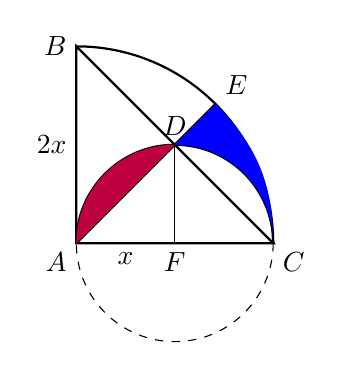
\begin{tikzpicture}[scale=0.5]
		\draw[thick] (0,5) -- (0,0) -- (5,0) -- cycle;
		\draw[thick] (5,0) arc (0:90:5);
		\draw[dashed] (5,0) arc (360:180:2.5);
		\draw[thick] (3.5355339,3.5355339) -- (0,0);
		\draw[thick] (5,0) arc (0:180:2.5);
		
		\path[fill=purple] (0,0) to [out=90,in=180] (2.5,2.5);
		\path[fill=blue] (3.5355339,3.5355339) to (2.5,2.5) to [out=0,in=90] (5,0) to [out=90,in=315] (3.5355339,3.5355339);
		
		\node[below left] at (0,0) {$A$};	
		\node[left] at (0,5) {$B$};
		\node[below right] at (5,0) {$C$};
		\node[above] at (2.5,2.5) {$D$};
		\node[above right] at (3.5355339,3.5355339) {$E$};
		\node[below] at (1.25,0) {$x$};
		\node[left] at (0,2.5) {$2x$};
		
		\draw (2.5,2.5) -- (2.5,0);
		\node[below] at (2.5,0) {$F$};
		\end{tikzpicture}
	\end{center}
	
	% Reasoning
	\paragraph{Reasoning}
	\begin{quotation}
		
		Mark the midpoint of $\overline{AC}$ as $F$, and draw $\overline{DF}$. Let $FA$ be $x$. Since the endpoints of a semicircle lie on a diameter according to the textbook's definition for a semicircle (6), $\overline{AC}$ is a diameter of the semicircle. Since the midpoint of a diameter is the center of the circle containing the semicircle, $F$ is the circle's center and is therefore equidistant from all points on the circle by definition. Since $A$, $D$, and $C$ lie on the semicircle that is contained by the circle, they are equidistant from $F$; thus $FA=FD=FC=x$ and $\overline{FA}\cong\overline{FD}\cong\overline{FC}$. By the SAP, $AF+FC=AC$; after substitution, $x+x=AC$ and therefore $2x=AC$. Given that $AC=AB$, $AB=2x$ by the Transitive Property. Since $\angle ADC$ is an inscribed angle of circle $F$ that subtends the imaginary semicircle in it (illustrated above as a dashed arc), $\angle ADC$ is a right angle and has a measure of 90\textdegree \space by definition (11). Since $D$ lies on $\overline{BC}$, $\text{m}\angle CDB=180$\textdegree \space by the Straight Angle Theorem. $\text{m}\angle ADC+\text{m}\angle ADB=\text{m}\angle CDB$ by the Angle Addition Postulate; after substitution, $90+\text{m}\angle ADB=180$; after subtracting 90 from both sides, $\text{m}\angle ADB=180-90=90$\textdegree. Since both $\angle ADC$ and $\angle ADB$ have a measure of 90\textdegree, $\angle ADB\cong\angle ADC$. Given that $AB=AC$, $\overline{AB}\cong\overline{AC}$ by definition. Since two sides of $\triangle ABC$ are congruent, the angles opposite these sides are also congruent ($\angle ABC\cong\angle ACB$) by the Isosceles Triangle Theorem. $\overline{AD}\cong\overline{AD}$ by the Reflexive Property. With two angles and a non-included side congruent, $\triangle ADB\cong\triangle ADC$ by AAS (5). Thus $\angle BAD\cong\angle CAD$ and $\overline{DB}\cong\overline{DC}$ by CPCTC. Since $\overrightarrow{AE}$ divides $\angle BAC$ into two congruent angles, it is an angle bisector by definition (1). By the Angle Addition Postulate, m$\angle BAD+\text{m}\angle CAD=\text{m}\angle BAC$. Given that m$\angle BAC=90$\textdegree \space and with m$\angle BAD=\text{m}\angle CAD$, $\text{m}\angle BAD=\text{m}\angle CAD=\frac{\text{m}\angle BAC}{2}=\frac{90}{2}=45$\textdegree. According to the Triangle Sum Theorem (3), $\text{m}\angle CAD+\text{m}\angle ADC+\text{m}\angle ACD=180$\textdegree; after substitution, $45+90+\text{m}\angle ACD=135+\text{m}\angle ACD=180$; when 135 is subtracted from both sides, $\text{m}\angle ACD=180-135=45$\textdegree. Thus $\text{m}\angle ACD=\text{m}\angle CAD$ by the Transitive Property; $\angle ACD\cong\angle CAD$ by definition. With this known, $\overline{AD}\cong\overline{CD}$ by the Converse of the Isosceles Triangle Theorem. Having two sides and their included angle congruent, $\triangle FAD\cong\triangle FCD$ by SAS (4). Thus $\angle AFD\cong\angle CFD$ by CPCTC and $\text{m}\angle AFD=\text{m}\angle CFD$ by the definition of angle congruence. Since $F$ lies on $\overline{AC}$, $\text{m}\angle AFC=180$\textdegree \space by the Straight Angle Theorem. By the Angle Addition Postulate, $\text{m}\angle AFD+\text{m}\angle CFD=\text{m}\angle AFC=180$\textdegree. Thus $\text{m}\angle AFD=\text{m}\angle CFD=\frac{\text{m}\angle AFC}{2}=\frac{180}{2}=90$\textdegree. Since $\widehat{AD}$ is a minor arc, its measure equals the measure of its central angle, $\angle AFD$ (6); therefore m$\widehat{AD}=\text{m}\angle AFD=90$\textdegree.
		
		The {\color{purple} purple} region illustrated above is a segment of a circle by definition (9), and its area can be determined by subtracting the area of $\triangle AFD$ from the area of sector $AFD$ (10). The area formula for a triangle is $\frac{1}{2}bh$ where $b$ is its base and $h$ is its height (2); after substitution, $[\triangle AFD]=\frac{1}{2}(x)(x)=\frac{1}{2}x^2$. The area formula for a sector of a circle is $r^2\pi(\frac{m\text{\textdegree}}{360\text{\textdegree}})$ where $r$ is the circle's radius and $m$ is the measure of its central angle (8); after substitution, $[\text{sector  } AFD]=x^2\pi (\frac{90}{360})=x^2\pi\frac{1}{4}$. The area of the {\color{purple} purple} region is therefore $[\text{sector  } AFD]-[\triangle AFD]=x^2\pi\frac{1}{4}-\frac{1}{2}x^2=x^2(\frac{1}{4}\pi-\frac{1}{2})$. Since $\overline{AD}\cong\overline{CD}$ (congruent chords), $\widehat{AD}\cong\widehat{CD}$ (congruent arcs) (7). Since congruent arcs have congruent central angles and equal radii, their corresponding segments (of circles) have the same area; therefore $[\text{\color{purple} purple region}]=[\text{segment  } AD]=[\text{segment  } CD]=x^2(\frac{1}{4}\pi-\frac{1}{2})$.
		
		By the Area Addition Postulate, $[\text{sector  } EAC]=[\text{\color{blue} blue region}]+[\text{segment  } CD]+[\triangle FCD]+[\triangle FAD]$. Since $\triangle FCD\cong\triangle FAD$, their areas are equal; therefore $[\triangle FCD]=[\triangle FAD]=\frac{1}{2}x^2$ and $[\triangle FCD]+[\triangle FAD]=\frac{1}{2}x^2+\frac{1}{2}x^2=x^2$. The central angle of sector $EAC$ is $\angle EAC$, whose measure is determined to equal 45\textdegree. Since a sector of a circle is bounded by two radii and its intercepted arc, and since $\overline{AE}$ and $\overline{AC}$ are the segments by which sector $EAC$ is bounded, $\overline{AE}$ and $\overline{AC}$ are its radii. Since $AC=2x$, the radius of the circle containing sector $EAC$ is $2x$. The area formula for a sector of a circle is $r^2\pi(\frac{m\text{\textdegree}}{360\text{\textdegree}})$ where $r$ is the circle's radius and $m$ is the measure of its central angle (8); after substitution, $[\text{sector  } EAC]=(2x)^2\pi(\frac{45}{360})=4x^2\pi\cdot\frac{1}{8}=\frac{4}{8}x^2\pi=\frac{1}{2}x^2\pi$.
		
		After substituting known terms for their values in the equation derived using the Area Addition Postulate above, $\frac{1}{2}x^2\pi=[\text{\color{blue} blue region}]+x^2(\frac{1}{4}\pi-\frac{1}{2})+x^2$. This is solved for $[\text{\color{blue} blue region}]$ as follows:
		
		\begin{center}
			\begin{tabular}{l | l}
				$\frac{1}{2}x^2\pi-x^2(\frac{1}{4}\pi-\frac{1}{2})-x^2=[\text{\color{blue} blue region}]$ & Subtract both sides by $(x^2(\frac{1}{4}\pi-\frac{1}{2})+x^2)$ \\
				$x^2(\frac{1}{2}\pi-(\frac{1}{4}\pi-\frac{1}{2})-1)=[\text{\color{blue} blue region}]$ & Apply the Distributive Property \\
				$x^2(\frac{1}{2}\pi-\frac{1}{4}\pi+\frac{1}{2}-1)=[\text{\color{blue} blue region}]$ & Reduce inner parentheses \\
				$x^2(\frac{1}{4}\pi-\frac{1}{2})=[\text{\color{blue} blue region}]$ & Simplify
			\end{tabular}
		\end{center}
	\end{quotation}
	
	Recall that the area of the {\color{purple} purple} region was derived to be the same expression ($[\text{\color{purple} purple region}]=x^2(\frac{1}{4}\pi-\frac{1}{2})$). Since $[\text{\color{blue} blue region}]=[\text{\color{purple} purple region}]$ by the Transitive Property, the ratio between them is $\boxed{1:1}$.
	
	\paragraph{External References}
	
	\begin{enumerate}
		\item Textbook Ch. 1, Pg. 23: Definition of an Angle Bisector
		\item Textbook Ch. 1, Pg. 36: Perimeter and Area of a Triangle
		\item Textbook Ch. 4, Pg. 223: Triangle Sum Theorem
		\item Textbook Ch. 4, Pg. 243: Side-Angle-Side Congruence
		\item Textbook Ch. 4, Pg. 254: Angle-Angle-Side Congruence
		\item Textbook Ch. 11, Pg. 756: Arcs and Their Measure (Definition of a Semicircle)
		\item Textbook Ch. 11, Pg. 757: In a circle, congruent chords have congruent arcs
		\item Textbook Ch. 11, Pg. 764: Sector of a Circle
		\item Textbook Ch. 11, Pg. 765: Definition of a Segment of a Circle
		\item Textbook Ch. 11, Pg. 765: Area of a Segment of a Circle
		\item Textbook Ch. 11, Pg. 774: Inscribed $\angle$ subtends semicircle  $\leftrightarrow$ Inscribed $\angle$ is a right $\angle$ 
	\end{enumerate}
	
\end{document}